\documentclass[xcolor={svgnames}]{beamer}

\setbeameroption{hide notes} 

%\usetheme{NLP}
\usetheme{boxes}
\useoutertheme{infolines}

\usepackage{graphicx}
\usepackage{lmodern}
\usepackage{calc}

\usepackage{soul}

\usepackage{amsmath,amsthm,amssymb}   

\usepackage{listings}
\usepackage[style=authoryear,babel=hyphen]{biblatex}
\addbibresource{ref.bib}
\addbibresource{pliang.bib}

%\usepackage{algorithm,algorithmic}

\usepackage{tikz}
%\usepackage[debug]{scabslides}
\usepackage{scabslides}

\usepackage{mathtools}

% Text
\newcommand{\todo}[1]{\hl{\textbf{TODO:} #1}}
\newcommand{\citationneeded} {\ensuremath{^{[\textrm{citation needed}]}}}


%Math Operators
%\DeclareMathOperator {\argmax} {argmax}
%\DeclareMathOperator {\argmin} {argmin}
\DeclareMathOperator {\sgn} {sgn}
\DeclareMathOperator {\trace} {tr}
\DeclareMathOperator{\E} {\mathbb{E}}
\DeclareMathOperator{\Var} {Var}
\DeclareMathOperator{\diag} {diag}
\DeclareMathOperator{\triu} {triu}
\DeclareMathOperator{\mult} {Multinomial}
\DeclareMathOperator{\normalt} {Normal}
\DeclareMathOperator{\cvec} {cvec}

\newcommand{\ud}{\, \mathrm{d}}
\newcommand{\diff}[1] {\frac{\partial}{\, \partial #1}}
\newcommand{\difff}[2] {\frac{\partial^2}{\, \partial #1\, \partial #2}}
\newcommand{\diffn}[2] {\frac{\partial^{#2}}{\, \partial {#1}^{#2}}}
\newcommand{\tuple}[1] {\langle #1 \rangle}
\newcommand{\innerprod}[2] {\langle #1, #2 \rangle}

% Constants/etc.
\renewcommand{\Re} {\mathbb{R}}
\newcommand{\Cm} {\mathbb{C}}
\newcommand{\Qm} {\mathbb{Q}}
\newcommand{\half} {\frac{1}{2}}

\newcommand{\inv}[1] {{#1}^{-1}}

\newcommand{\normal}[2] {\mathcal{N}(#1, #2)}
\newcommand{\mL} {\mathcal{L}}

\newcommand\eqdef{\ensuremath{\stackrel{\rm def}{=}}} % Equal by definition
\newcommand\refeqn[1]{(\ref{eqn:#1})}
\newcommand\sD{\ensuremath{\mathcal{D}}}
\newcommand\sM{\ensuremath{\mathcal{M}}}
\newcommand\refapp[1]{Appendix~\ref{sec:#1}}
\newcommand\refthm[1]{Theorem~\ref{thm:#1}}
\newcommand\sigmamin{\sigma_\text{\rm min}}
\newcommand\sigmamax{\sigma_\text{\rm max}}
\newcommand\op{{\text{\rm op}}}
\newcommand\BP{\ensuremath{\mathbb{P}}}
\newcommand\reflem[1]{Lemma~\ref{lem:#1}}

% Tensor powers
\newcommand{\tp}[1] {^{\otimes #1}}

% Matrix Perturbation
\newcommand{\pinv}[1] {#1^{\dagger}}
\newcommand{\Ap} {\hat{A}}
\newcommand{\Bp} {\hat{B}}
\newcommand{\Up} {\hat{U}}
\newcommand{\Vp} {\hat{V}}
\newcommand{\Xp} {\hat{X}}
\newcommand{\Wp} {\hat{W}}
\newcommand{\cM} {\mathcal{M}}
\newcommand{\cMp} {\hat{\mathcal{M}}}
\newcommand{\Mp} {\hat{M}}
\newcommand{\Zp} {\hat{Z}}
\newcommand{\vp} {\hat{v}}
\newcommand{\lambdap} {\hat{\lambda}}
\newcommand{\sigmap} {\hat{\sigma}}
\newcommand{\mup} {\hat{\mu}}
\newcommand{\cnd}[1] {\kappa(#1)}
\newcommand{\aerr}[1] {\varepsilon_{#1}}
\newcommand{\rerr}[1] {\delta_{#1}}
\newcommand{\serr}[1] {\alpha_{#1}}
\newcommand{\berr}[1] {\beta_{#1}}
\newcommand{\gap}[1] {\Delta_{#1}}

% Keywords
\newcommand{\Pairs}{\mathrm{Pairs}}
\newcommand{\Triples}{\mathrm{Triples}}



\newcommand<>{\drawgen}[1]{%
  \uncover#2{
    \point{start-gen}{#1}
    \node[style=node] (h) at (start-gen) {};
    \node[left=0.1cm of h] {$h$};
    \node[style=node,fill=green!70,below=1cm of h] (x) {};
    \node[left=0.1cm of x] {$x$};
    \draw[-latex] (h) -- (x);
  }
}

\newcommand<>{\drawdisc}[1]{%
  \uncover#2{
    \point{start-disc}{#1}
    \node[style=node] (h) at (start-disc) {};
    \node[right=0.1cm of h] {$h$};

    \node[style=obsnode,left=0.3cm of h] (x) {};
    \node[left=0.1cm of x] {$x$};

    \node[style=obsnode,below=1cm of h] (y) {};
    \node[left=0.1cm of y] {$y$};
    \draw[-latex] (h) -- (y);
    \draw[-latex] (x) -- (y);
  }
}

\newcommand{\tensorfactorization}[1]{%
  \point{start-tf}{#1}
  \tikzcube{tensoring}{black,fill=white}{($(start-tf) + (0,0,0)$)}{1}{1}{1};
  \node at ($(tensoring) + (1.0cm,-0.3cm)$) {$=$};
  \tensorfiber{t1}{fill=blue!70}{($(tensoring) + (2.5cm,0.0cm)$)};
  \node at ($(t1) + (1.0cm,-0.3cm)$) {$+$};
  \tensorfiber{t2}{fill=green!70}{($(t1) + (2.5cm,0.0cm)$)};
  \node at ($(t2) + (1.0cm,-0.3cm)$) {$+ \dots + $};
  \tensorfiber{t3}{fill=red!70}{($(t2) + (3.0cm,0.0cm)$)};

  \draw [decorate,decoration={brace,amplitude=10pt,raise=4pt,mirror},yshift=0pt] 
    ($(t1) + (-1cm,-1cm)$) -- ($(t3) + (0.2cm,-1cm)$) node [below,black,midway,yshift=-0.6cm] {$k$};
}

\newcommand{\matrixfactorization}[1]{%
    \point{start-mf}{#1}
    \tikzrect{mat}{black,fill=white}{($(start-mf) + (0,0)$)}{1}{1};
    \node at ($(mat) + (1.0cm,-0.3cm)$) {$=$};
    \matfiber{t1}{fill=blue!70}{($(mat) + (2.5cm,0.0cm)$)};
    \node at ($(t1) + (1.0cm,-0.3cm)$) {$+$};
    \matfiber{t2}{fill=green!70}{($(t1) + (2.5cm,0.0cm)$)};
    \node at ($(t2) + (1.0cm,-0.3cm)$) {$+ \dots + $};
    \matfiber{t3}{fill=red!70}{($(t2) + (3.0cm,0.0cm)$)};
    \draw [decorate,decoration={brace,amplitude=10pt,raise=4pt,mirror},yshift=0pt] 
      ($(t1) + (-1cm,-1cm)$) -- ($(t3) + (0.2cm,-1cm)$) node [below,black,midway,yshift=-0.6cm] {$k$};
}

\newcommand{\llhood}[2]{%
  \begin{axis}[
      x=1cm,
      y=3cm,
      scale only axis,
      height=8cm,
      width=4cm,
      axis lines*=left,
      xtick=\empty,
      ytick=\empty,
      xlabel=$\theta$,
      ylabel=$-\log p_{\theta}(x)$
      ]
    \addplot[
        black,
        thick,
        smooth,
        ] file [% Provide data as a table
          ] {data/llhood.table}
     node[pos=0.27] (em1) {}
     node[pos=0.5] (spec) {}
     node[pos=0.61] (mle) {}
     node[pos=0.85] (em2) {}
     node[pos=0.9] (em2-start) {}
     ;

  \end{axis}
}

\newcommand{\mog}[2]{%
    \begin{axis}[
        xshift=#1,
        yshift=#2,
        scale only axis,
        height=3cm,
        width=3cm,
        axis lines*=left,
        xlabel=$x_1$,
        ylabel=$x_2$,
        xtick=\empty,
        ytick=\empty,
        mark options={scale=0.2,line width=0}
        ]
      \addplot+[
          smooth,
          only marks
          ] file [% Provide data as a table
            ] {data/mog-0.table};
      \addplot+[
          smooth,
          only marks
          ] file [% Provide data as a table
            ] {data/mog-1.table};
      \addplot+[
          smooth,
          only marks
          ] file [% Provide data as a table
            ] {data/mog-2.table}
       ;

    \end{axis}
}

\newcommand{\innerpdiag}[2]{%
  \node[scale=2.0] at ($#1 + (-1.3cm,-0.3cm)$) {$\langle$};
  \node at ($#1!0.5!#2 + (-0.3cm,-0.3cm) $) {$,$};
  \node[scale=2.0] at ($#2 + (0.8cm,-0.3cm)$) {$\rangle$};
}
\newcommand{\innerpdiagv}[2]{%
  \node[scale=2.0] at ($#1 + (-0.7cm,-0.45cm)$) {$\langle$};
  \node at ($#1!0.5!#2 + (-0.1cm,-0.45cm) $) {$,$};
  \node[scale=2.0] at ($#2 + (0.4cm,-0.45cm)$) {$\rangle$};
}
\newcommand{\innerpdiagm}[2]{%
  \node[scale=2.0] at ($#1 + (-1.3cm,-0.45cm)$) {$\langle$};
  \node at ($#1!0.5!#2 + (-0.5cm,-0.45cm) $) {$,$};
  \node[scale=2.0] at ($#2 + (0.4cm,-0.45cm)$) {$\rangle$};
}
\newcommand{\innerpdiagt}[2]{%
  \node[scale=2.0] at ($#1 + (-1.3cm,-0.3cm)$) {$\langle$};
  \node at ($#1!0.5!#2 + (-0.3cm,-0.3cm) $) {$,$};
  \node[scale=2.0] at ($#2 + (0.7cm,-0.3cm)$) {$\rangle$};
}

\newcommand{\regressionA}[1]{%
    \point{start-reg-a}{#1};
    \point{start-reg-a-A}{(start-reg-a)};
    \point{start-reg-a-B}{($(start-reg-a) + (1cm,0) $)};

    \tikzrect{A}{black,fill=yellow}{($(start-reg-a-A) + (0,0)$)}{0.3}{1};
    \tikzrect{B}{black,fill=blue!70}{($(start-reg-a-B) + (0,0)$)}{0.3}{1};
    \innerpdiagv{(start-reg-a-A)}{(start-reg-a-B)};
}

\newcommand{\regressionB}[1]{%
    \point{start-reg-b}{#1};
    \point{start-reg-b-A}{(start-reg-b)};
    \point{start-reg-b-B}{($(start-reg-b) + (1.5cm,0) $)};

    \tikzrect{A}{black,fill=yellow}{($(start-reg-b-A) + (0,0)$)}{1}{1};
    \tikzrect{B}{black,fill=blue!70}{($(start-reg-b-B) + (0,0)$)}{1}{1};
    \innerpdiagm{(start-reg-b-A)}{(start-reg-b-B)};
}

\newcommand{\regressionC}[1]{%
    \point{start-reg-c}{#1};
    \point{start-reg-c-A}{(start-reg-c)};
    \point{start-reg-c-B}{($(start-reg-c) + (1.8cm,0) $)};

    \tikzcube{A}{black,fill=yellow}{($(start-reg-c-A) + (0,0)$)}{1}{1}{1};
    \tikzcube{B}{black,fill=blue!70}{($(start-reg-c-B) + (0,0)$)}{1}{1}{1};
    \innerpdiagt{(start-reg-c-A)}{(start-reg-c-B)};
}


\newcommand{\mkmlrplot}[3]{%
\begin{tikzpicture}
\begin{axis}[ 
    xshift=#1, 
    yshift=#2, 
    height=5cm, width=5cm, 
    axis lines*=left, 
    xlabel=$x$, ylabel=$y$, 
    xtick=\empty, ytick=\empty, 
    mark options={scale=0.3,line width=0},
    xmin=-1.2, xmax=1.2,
    ]
  #3
\end{axis}
\end{tikzpicture}
}


\newcommand{\mlrfull}[2]{%
  \only<1>{%
    \mkmlrplot{#1}{#2}{%
       \addplot+[blue, line width=2pt, mark=none] {0.316 + -0.862*x};
       \addplot+[green,line width=2pt, mark=none] {-0.715 + -0.268*x};
       \addplot+[red,  line width=2pt, mark=none] {-1.076 + 0.595*x};
     }
  }
  \only<2>{%
    \mkmlrplot{#1}{#2}{%
       \addplot+[blue,                 mark=none] {0.316 + -0.862*x};
       \addplot+[green,                mark=none] {-0.715 + -0.268*x};
       \addplot+[red,  line width=2pt, mark=none] {-1.076 + 0.595*x};
     }
  }
  \only<3>{%
    \mkmlrplot{#1}{#2}{%
       \addplot+[blue,                 mark=none] {0.316 + -0.862*x};
       \addplot+[green,                mark=none] {-0.715 + -0.268*x};
       \addplot+[red,  line width=2pt, mark=none] {-1.076 + 0.595*x};
       \addplot[smooth, black, only marks] table {data/mlr-1.table};
     }
  }
  \only<4>{%
    \mkmlrplot{#1}{#2}{%
       \addplot+[blue, line width=2pt, mark=none] {0.316 + -0.862*x};
       \addplot+[green,                mark=none] {-0.715 + -0.268*x};
       \addplot+[red,                  mark=none] {-1.076 + 0.595*x};
       \addplot[smooth, black, only marks] table {data/mlr-1.table};
     }
  }
  \only<5>{%
    \mkmlrplot{#1}{#2}{%
       \addplot+[blue, line width=2pt, mark=none] {0.316 + -0.862*x};
       \addplot+[green,                mark=none] {-0.715 + -0.268*x};
       \addplot+[red,                  mark=none] {-1.076 + 0.595*x};
       \addplot[smooth, black, only marks] table {data/mlr-2.table};
     }
  }
  \only<6>{%
    \mkmlrplot{#1}{#2}{%
       \addplot[smooth, black, only marks] table {data/mlr.table};
       \addplot+[blue, line width=2pt, mark=none] {0.316 + -0.862*x};
       \addplot+[green,line width=2pt, mark=none] {-0.715 + -0.268*x};
       \addplot+[red,  line width=2pt, mark=none] {-1.076 + 0.595*x};
     }
  }
  \only<7>{%
    \mkmlrplot{#1}{#2}{%
       \addplot[smooth, black, only marks] table {data/mlr.table};
     }
  }
}

\newcommand{\mlrdata}[2]{%
    \mkmlrplot{#1}{#2}{%
     \addplot[smooth, black, only marks] table {data/mlr.table};
   }
}



% these will be used later in the title page
\title[Spectral Experts]{Spectral Experts for Estimating Mixtures of Linear Regressions}
\author[Chaganty, Liang]{%
    Arun Tejasvi Chaganty\\
    Percy Liang
}
\institute{Stanford University}

\begin{document}

% "Beamer, do the following at the start of every section"
\AtBeginSection[] 
{%
\begin{frame}<beamer> 
\frametitle{Outline} % make a frame titled "Outline"
\tableofcontents[currentsection]  % show TOC and highlight current section
\end{frame}
}

\begin{frame}
  \titlepage
\end{frame}

\begin{frame}
  \frametitle{Latent Variable Models}

  \splitcolumn{%
    \begin{itemize} 
      \item {\bf Generative Models} \tikzmark{gen}
        \uncover<2->{%
        \begin{itemize}
          \item Gaussian Mixture Models
          \item Hidden Markov Models
          \item Latent Dirichlet Allocation
          \item PCFGs
          \item \dots
        \end{itemize}
        }
      \item<3-> {\bf Discriminative Models} \tikzmark{disc}
        \uncover<4->{%
        \begin{itemize}
          \item Mixture of Experts
          \item Latent CRFs
          \item Discriminative LDA
          \item \dots
          \item {\em Easy to include features and tend to be more accurate.}
        \end{itemize}
        }
      \end{itemize}
  }{%
  \begin{canvas}
    \point{mark}{(3cm,0)};
    \point{gen}{({pic cs:gen} -| mark)}
    \point{disc}{({pic cs:disc} -| mark)}
    \node<1->[anchor=north east] at ($(gen) +(0,1.0cm)$) {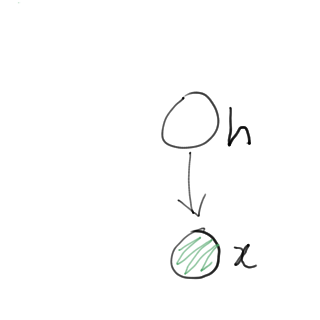
\includegraphics[width=\textwidth,height=2cm,keepaspectratio]{figures/gen.png}};
    \node<3->[anchor=north east] at ($(disc) +(0,-0.5cm)$) {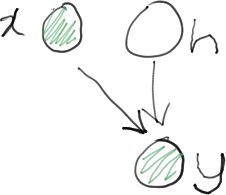
\includegraphics[width=\textwidth,height=2cm,keepaspectratio]{figures/disc.png}};
  \end{canvas}
  }

\end{frame}

\begin{frame}
  \frametitle{Parameter Estimation is Hard}

  \begin{tikzpicture}
    % x, y
    \node at (0,0) {%
    \includegraphics<1>[width=\textwidth,height=6cm,keepaspectratio]{figures/likelihood.png}
    \includegraphics<2>[width=\textwidth,height=6cm,keepaspectratio]{figures/likelihood-mle.png}
    \includegraphics<3>[width=\textwidth,height=6cm,keepaspectratio]{figures/likelihood-em.png}
    \includegraphics<4>[width=\textwidth,height=6cm,keepaspectratio]{figures/likelihood-mom.png}
      };
    %\point{opt}{(0.4cm,-1.1cm)};
    %\node[style=lbl,below=0.0cm of opt,scale=1.2] {$\hlmath{blue}{\theta^*}$};
    % Axes
    \draw[-latex] (-6cm,-2.25cm) -- node[right,at end]{$-\log(p_{\theta}(x))$}  (-6cm,2cm);
    \draw[-latex] (-6cm,-2.25cm) -- node[above,at end]{$\theta$}  (5cm,-2.25cm);
  \end{tikzpicture}

  % Simple message: MLE is consistent but intractable, EM is efficient not but consistent. Can we get something in between.

  \begin{itemize}
    \item<1-> Log-likelihood function is non-convex.
    \item<2-> MLE is consistent but intractable.
    \item<3-> Local methods (EM, gradient descent, etc.) are tractable but inconsistent.
    \item<4-> Can we build {\bf efficient yet consistent estimators} that get better with more data?
  \end{itemize}

\end{frame}

\begin{frame}
  \frametitle{Related Work}
  \begin{itemize}
    \item<1-> Method of Moments [Pearson, 1894]
    \item<2-> Observable operator models
    \begin{itemize}
      \item Control Theory [Ljung, 1987]
      \item Observable operator models [Jaeger, 2000; Singh et al., 2004]
      \item \alert<2>{Hidden Markov models [Hsu et al, 2009]}
      \item Low-treewidth graphs [Parikh et al., 2012]
      \item Weighted finite state automata [Balle \& Mohri, 2012]
    \end{itemize}
     \item<3-> Parameter Estimation
  \begin{itemize}
    \item Mixture of Gaussians [Kalai/Moitra/Valiant, 2010]
    \item \alert{Mixture models, HMMs [Anandkumar/Hsu/Kakade, 2012]}
    \item Latent Dirichlet Allocation [Anandkumar/Hsu/Kakade, 2012]
    \item Stochastic block models [Anandkumar/Ge/Hsu/Kakade, 2012]
    \item Linear Bayesian networks [Anandkumar/Hsu/Javanmard/Kakade, 2012]
  \end{itemize}
  \end{itemize}
\end{frame}

\begin{frame}
  \frametitle{Aside: Tensor Operations}
  \splitcolumn{%
    \begin{itemize}
      \item \tikzmark{tensoring} Tensoring
        $$x\tp{3}_{ijk} = x_i x_j x_k$$
      \item \tikzmark{innerp}Inner product
        \begin{align*}
          \innerp{A}{B} &= \sum_{ijk} A_{ijk} B_{ijk} \\
          \pause
            &= \innerp{\vvec{A}}{\vvec{B}} 
        \end{align*}
    \end{itemize}
  }{%
  }
  \begin{canvas}
    \point{mark}{(6.8cm,0)};
    % Tensoring
    \tikzcube{tensoring}{black,fill=white}{($({pic cs:tensoring} -| mark) + (0,0,0)$)}{1}{1}{1};
    \node at ($(tensoring) + (1.0cm,-0.3cm)$) {$=$};
    \tikzcube{v1}{black,fill=white}{($(tensoring) + (2.5cm,-0.3cm)$)}{1}{0.3}{0.3};
    \node (lbl1) at ($(v1) + (0.40cm,-0.1cm)$) {$\times$};
    \tikzcube{v2}{black,fill=white}{($(v1) + (1cm,0.3cm)$)}{0.3}{1}{0.3};
    \node at ($(lbl1) + (1cm,0.0cm)$) {$\times$};
    \tikzcube{v3}{black,fill=white}{($(v2) + (1cm,-0.3cm)$)}{0.3}{0.3}{1};

    % Inner product
    \uncover<2->{%
    \point{ptA}{($({pic cs:innerp} -| mark) + (0,0.2cm)$)}
    \point{ptB}{($(ptA) + (2cm,0)$)}
    \tikzcube{innerpA}{black,fill=yellow}{($(ptA) + (0,0,0)$)}{1}{1}{1};
    \tikzcube{innerpB}{black,fill=blue,opacity=0.7}{($(ptB) + (0,0,0)$)}{1}{1}{1};
    \node[scale=2.0] (op1a) at ($(ptA) + (-1.3cm,-0.3cm)$) {$\langle$};
    \node (op1b) at ($(ptA) + (0.7cm,-0.3cm)$) {$,$};
    \node[scale=2.0] (op1c) at ($(ptB) + (0.8cm,-0.3cm)$) {$\rangle$};
    \node[scale=2.0] (op2) at ($(op1c) + (1.5cm,0.0cm)$) {$= \hlmath{green}{0.5}$};
    }

    % Inner product 2
    \uncover<3->{%
    \tikzrect{innerpAv}{black,fill=yellow}{($(ptA) + (0,-1.5cm)$)}{0.3}{1.5};
    \tikzrect{innerpBv}{black,fill=blue,opacity=0.7}{($(ptB) + (0,-1.5cm)$)}{0.3}{1.5};
    \node[scale=2.0] (op1a) at ($(innerpAv) + (-1.3cm,-0.6cm)$) {$\langle$};
    \node (op1b) at ($(innerpAv) + (0.7cm,-0.6cm)$) {$,$};
    \node[scale=2.0] (op1c) at ($(innerpBv) + (0.8cm,-0.6cm)$) {$\rangle$};
    \node[scale=2.0] (op2) at ($(op1c) + (1.5cm,0.0cm)$) {$= \hlmath{green}{0.5}$};
    }
  \end{canvas}

\end{frame}

\begin{frame}
  \frametitle{Example: Gaussian Mixture Model}

  \splitcolumn{%
    \begin{itemize}
      \item \tikzmark{gen} Generative process:
      \begin{align*}
        h &\sim \Mult(\pi) \\
        x &\sim \normal{\beta_h}{\sigma^2}.
      \end{align*}
      \item Moments:
      \begin{align*}
          \uncover<2->{%
          \E[x|h] &= \beta_h \\
          }
          \uncover<3->{%
          \E[x] &= \sum_h \pi_h \beta_h \\
          }
          \uncover<4->{%
          \tikzmark{m2}
          \E[x\tp{2}] &= \sum_h \pi_h (\beta_h \beta_h^T) \\
                      &= \sum_h \pi_h \beta_h{\tp{2}} \\
                      }
          \uncover<5->{%
          \tikzmark{m3}
          \E[x\tp{3}] &= \sum_h \pi_h \beta_h\tp{3}.
          }
        \end{align*}
    \end{itemize}
  }{%
  }
  \begin{canvas}
    % The model
    \point{mark}{(6.5cm,0)};
    \point{start}{({pic cs:gen} -| mark)};
    \node[anchor=west] (diag1) at ($(start)$) {%
      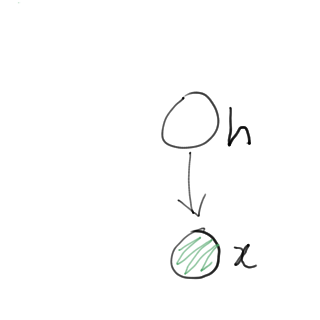
\includegraphics[width=0.45\textwidth,height=2cm,keepaspectratio]{figures/gen.png}
    };
    \node[anchor=west] (diag) at ($(start) + (1cm,0.0cm)$) {%
      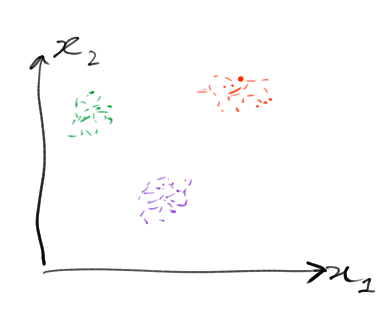
\includegraphics[width=0.45\textwidth,height=3cm,keepaspectratio]{figures/mog.png}
    };

    \uncover<4->{%
      \point{m2}{({pic cs:m2} -| mark)};
      \tikzrect{M2}{black,fill=white}{($(m2) + (1cm,1cm)$)}{1}{1};
      \node[anchor=west] at ($(m2) + (1.1cm, 0.5cm)$) {$\E[x\tp{2}]$};
      \node[anchor=east] at ($(m2) + (-0.1cm, 0.5cm)$) {$d$};
      \node[anchor=south] at ($(m2) + (0.5cm, 1.0cm)$) {$d$};
    }
    \uncover<5->{%
      \point{m3}{($({pic cs:m3} -| mark) + (1cm,1cm)$)};
      \tikzcube{M3}{black,fill=white}{($(m3) + (0,0,0)$)}{1}{1}{1};
      \node[anchor=west] at ($(m3) + (0.5cm, -0.5cm)$) {$\E[x\tp{3}]$};
      \node[anchor=east] at ($(m3) + (-1.1cm, -0.5cm)$) {$d$};
    }
  \end{canvas}

\end{frame}

\begin{frame}
  \frametitle{Solution: Tensor Factorization}
  \splitcolumn{%
    \begin{itemize}
      \item \tikzmark{gen}$\E[x\tp{3}] = \sum_{h=1}^k \pi_h \beta_h\tp{3}$.
      \item<2-> If $\beta_h$ are orthogonal, the are eigenvectors! \footcite{AnandkumarGeHsu2012}
        \begin{align*}
          \E[x\tp{3}](\beta_h,\beta_h) 
            %&= \sum_{h'=1}^k \pi_{h'} (\beta_{h}^T \beta_{h'})^2 \beta_{h'} \\
            %&= \sum_{h'=1}^k \pi_{h'} \delta_{hh'} \beta_{h'} \\
            &= \pi_{h} \beta_{h}.
        \end{align*}
      \item<3-> In general, whiten $\E[x\tp{3}]$ first.
    \end{itemize}
  }{%
  }
  \begin{canvas}
    \point{mark}{(6.5cm,0)};
    \point{start}{({pic cs:gen} -| mark)};

    \node[anchor=west] (diag1) at ($(start)$) {%
      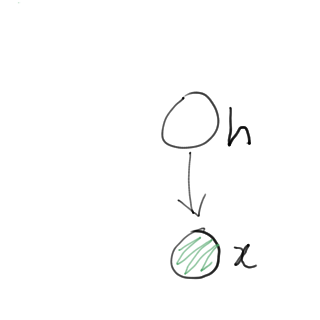
\includegraphics[width=0.45\textwidth,height=2cm,keepaspectratio]{figures/gen.png}
    };
    \node[anchor=west] (diag) at ($(start) + (1cm,0.0cm)$) {%
      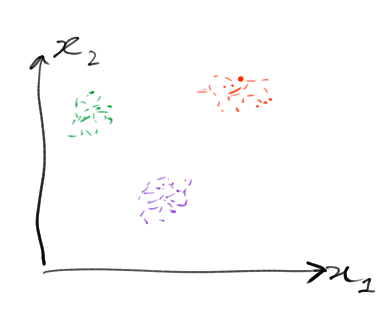
\includegraphics[width=0.45\textwidth,height=3cm,keepaspectratio]{figures/mog.png}
    };
    %\drawgen{(start)};
    %\node[anchor=west] (diag) at ($(start) + (1cm,-0.5cm)$) {%
    %  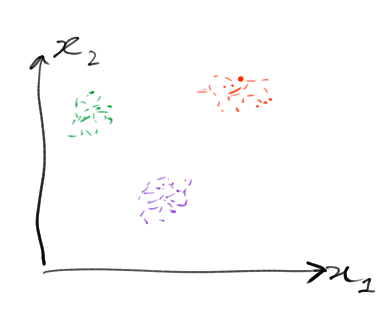
\includegraphics[width=0.45\textwidth,height=3cm,keepaspectratio]{figures/mog.png}
    %};
    % x, y
    %\node[anchor=north west] at ($(start) - (1cm,2cm)$) {%
    %    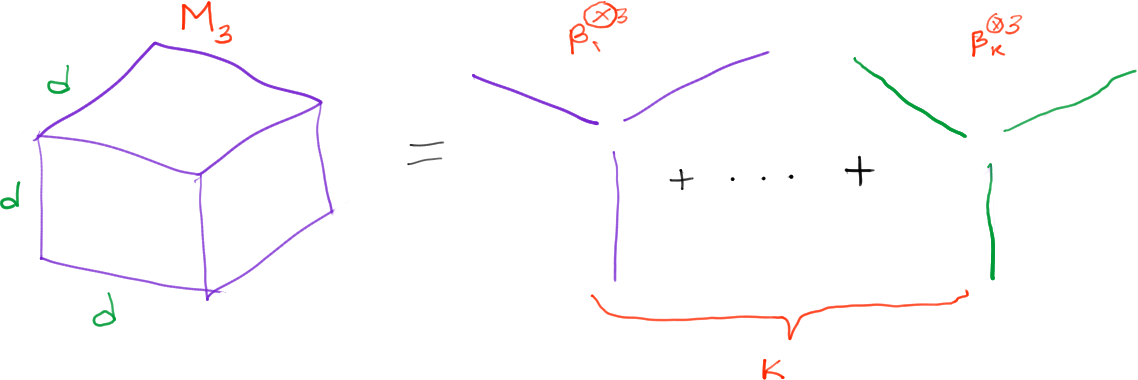
\includegraphics[width=6cm,height=2cm,keepaspectratio]{figures/tensor.png}
    %};
  \end{canvas}
\end{frame}

\begin{frame}
  \frametitle{}

  \begin{canvas}
    % Tasks.
    \node[anchor=west] (gen) at (1cm,0) {%
      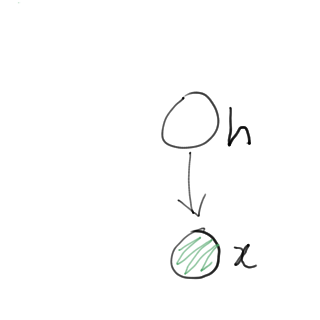
\includegraphics[width=\textwidth,height=2.5cm,keepaspectratio]{figures/gen.png}
     };
     \node[below=0.1cm of gen.south] {Generative Models};

    \draw[scale=0.8,fill=green,opacity=0.4,dashed] (6.5cm,2cm) rectangle (12.5cm,-3cm);
    \node[style=box,anchor=west] (disc) at (6cm,0) {%
      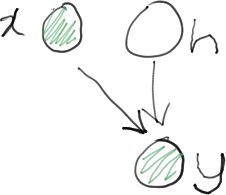
\includegraphics[width=\textwidth,height=3cm,keepaspectratio]{figures/disc.png}
     };
     \node[below=0.1cm of disc.south] {Discriminative Models};
     % Highlight
  \end{canvas}

\end{frame}


\begin{frame}
  \frametitle{Mixture of Linear Regressions}

  \splitcolumn{%
    \tikzmark{model}
    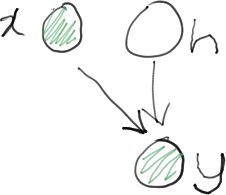
\includegraphics[width=3cm,height=4cm,keepaspectratio]{figures/disc.png}
    \begin{itemize}
      \item<2-> $h \sim \Mult(\pi)$.
      \item<4-> $y = \beta_h^T x + \epsilon$.
    \end{itemize}
  }{%
  }
    \begin{canvas}
      % x, y
      \point{mark}{(5.5cm,0)}
      \point{model}{({pic cs:model} -| mark)}
      \node[anchor=west] at ($(model) + (0,0.5cm)$) {%
      \includegraphics<1>[width=5cm,height=6cm,keepaspectratio]{figures/mlr-data-2.png}
      \includegraphics<2>[width=5cm,height=6cm,keepaspectratio]{figures/mlr-data-3a.png}
      \includegraphics<3>[width=5cm,height=6cm,keepaspectratio]{figures/mlr-data-3b.png}
      \includegraphics<4>[width=5cm,height=6cm,keepaspectratio]{figures/mlr-data-4a.png}
      \includegraphics<5>[width=5cm,height=6cm,keepaspectratio]{figures/mlr-data-4b.png}
      %\includegraphics<6>[width54cm,height=6cm,keepaspectratio]{figures/mlr-data-4c.png}
      \includegraphics<6>[width=5cm,height=6cm,keepaspectratio]{figures/mlr-data-5.png}
        };
    \end{canvas}
\end{frame}

\begin{frame}
  \frametitle{Mixture of Linear Regressions}

  \begin{canvas}
    \node[anchor=west] (data) at (0,0) {%
    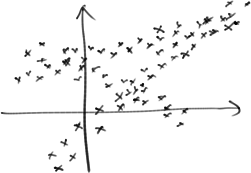
\includegraphics[width=4cm,height=6cm,keepaspectratio]{figures/mlr-data.png}
    };

    % x, y
    \node[anchor=west,scale=2.0] (params) at (7cm,0) {%
      $\begin{bmatrix} \pi \\ B \end{bmatrix}$
      };
    \node[anchor=west,right=0.1cm of params] {%
    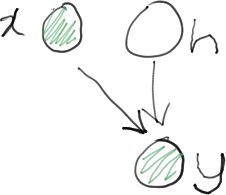
\includegraphics[width=4cm,height=2cm,keepaspectratio]{figures/disc.png}
    };

    \draw[-latex] (data) -- node[above]{?} (params);


  \end{canvas}
\end{frame}

% \begin{frame}
%   \frametitle{Method of Moments for Generative LVMs.}
% 
%   \begin{tikzpicture}
%     % x, y
%     \node<1->[style=box]  (moments) at (0,0) {\objw{12cm}{%
%       \begin{align*}
%         \underbrace{\E[x]}_{M_1} &= \sum_{h=1}^k \pi_h \beta_h & 
%         \underbrace{\E[x\tp{2}]}_{M_2} &= \sum_{h=1}^k \pi_h \beta_h\tp{2} & 
%         \underbrace{\E[x\tp{3}]}_{M_3} &= \sum_{h=1}^k \pi_h \beta_h\tp{3}. 
%       \end{align*}
%     }};
%     \node<1>[style=box,below=0.1cm of moments] {\objw{12cm}{%
%     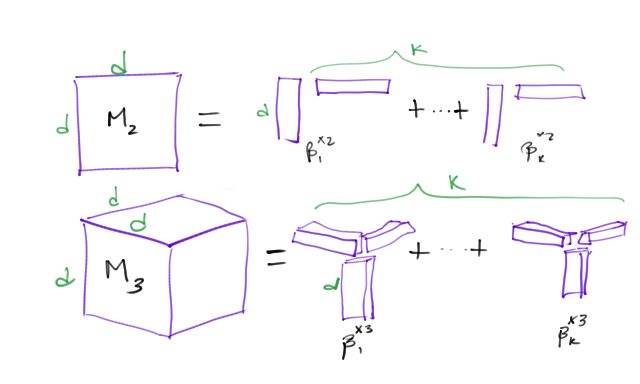
\includegraphics[width=\textwidth,height=6cm,keepaspectratio]{figures/moments.png}
%       }};
%     \node<2->[style=box,below=0.1cm of moments] {\objw{12cm}{%
%       \begin{itemize}
%         \item<2-> {\bf Tensor Power Method} for orthonormal $\beta_h$,
%           \begin{align*}
%             M_3(\beta_h,\beta_h) 
%               &= \sum_{h'=1}^k \pi_{h'} (\beta_{h}^T \beta_{h'})^2 \beta_{h'} \\
%               &= \sum_{h'=1}^k \pi_{h'} \delta_{hh'} \beta_{h'} \\
%               &= \pi_{h'} \beta_{h}.
%           \end{align*}
%         \item<3-> Use $M_2$ to whiten $M_3$.
%       \end{itemize}
%       }};
%   \end{tikzpicture}
% 
% \end{frame}

\begin{frame}[c]
  \frametitle{Method of Moments for the Mixture of Linear Regressions.}
  \begin{align*}
    y &= \alt<1>{\innerp{\beta_h}{x}}{\underbrace{\beta_h^T}_{\textrm{\color{DarkGreen}random}} x} + \epsilon \\
    \action<3->{%
    &= \sum_h \pi_h \innerp{\beta_h}{x} + \innerp{\left(\beta_h - \sum_h \pi_h \beta_h\right)}{x} + \epsilon \\
    }
    \action<4-6>{%
    &= \alt<4>{\E[\beta_h]^T x}{\underbrace{\E[\beta_h]^T x}_{\textrm{\color{blue}linear measurement}}} 
    + \alt<4-5>{\innerp{(\beta_h - \E[\beta_h])}{x} + \epsilon}{\underbrace{\innerp{(\beta_h - \E[\beta_h])}{x} + \epsilon}_{\textrm{\color{red} noise}}} \\
    }
  \end{align*}
\end{frame}

\begin{frame}
  \frametitle{Method of Moments for the Mixture of Linear Regressions.}

  \begin{align*}
    \action<1->{%
    y &= \overbrace{\innerp{\E[\beta_h]}{x}}^{\textrm{\color{blue} linear measurement}} & & + \overbrace{(\beta_h - \E[\beta_h])^T x + \epsilon}^{\textrm{\color{red} noise}} \\
    }
    \action<2->{%
      y^2 
      &= \innerp{\beta_h}{x}^2 &+ \epsilon^2 &+ 2 \epsilon \innerp{\beta_h}{x}  \\
    }
    \action<3->{%
      &= \color{blue}\innerp{\E[\beta_h\tp{2}]}{x\tp{2}} &+ \color{DarkGreen} \textrm{bias} &+ \color{red} \textrm{noise} \\
    }
    \action<4->{%
    y^3 &= \color{blue} \innerp{\E[\beta_h\tp{3}]}{x\tp{3}} &+ \color{DarkGreen} \textrm{bias} &+ \color{red} \textrm{noise} \\
    }
  \end{align*}

  %\begin{tikzpicture}
  %  % x, y
  %  \node<5->[style=box] (tensor) {\objw{12cm}{%
  %    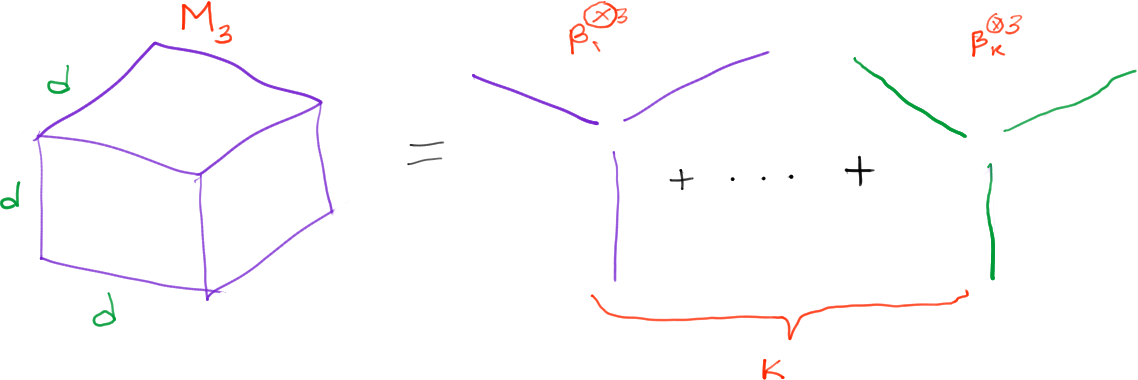
\includegraphics[width=\textwidth,height=3cm,keepaspectratio]{figures/tensor.png}
  %    }};
  %\end{tikzpicture}
\end{frame}

\begin{frame}
  \frametitle{Method of Moments for the Mixture of Linear Regressions.}
  \centering
  
  \begin{itemize}
  {\Large
    \item 
    $\E[\beta_h\tp{3}] = \sum_{h=1}^k \pi_h \beta_h\tp{3}$
  }
    \item<2-> Apply tensor factorization!
  \end{itemize}
\end{frame}

\begin{frame}
  \frametitle{Overview: Spectral Experts}

  \begin{canvas}
    % x, y
% Nodes
%\node[style=txt,anchor=south west] (data1) at (1cm,1cm) {$\left\{ x, y \right\}_{(x,y) \in \sD}$};
\node[style=txt] (data2) at (-4cm,1cm) {$\left\{ x\tp{2}, y^2 \right\}_{(x,y) \in \sD}$};
\node[style=txt,below=1cm of data2.center] (data3) {$\left\{ x\tp{3}, y^3 \right\}_{(x,y) \in \sD}$};

%\node[style=txt,anchor=south west] (m1) at (2cm,1cm) {$\E\left[\beta_h\right]$};
\node[style=txt] (m2) at (0cm,1cm) {$M_2$}; %{$\E\left[\beta_h\tp{2}\right]$};
\node[style=txt,below=1cm of m2.center] (m3) {$M_3$}; %{$\E\left[\beta_h\tp{3}\right]$};

\node[below=0.5cm of m2.center] (params-pos) {};
\node[style=txt,right=3.0cm of params-pos] (params) {$\pi, B$};

% Arrows
%\draw[-latex] (data1) -- (m1);
\draw[-latex] (data2) -- (m2);
\draw[-latex] (data3) -- (m3);

% Bias influence
%\draw[-latex,dashed,gray] (m1.east) -- ++(0.1cm,0) -- ++(0,-0.50cm) -- ++(-3.00cm,0) node (bias-1) {} -- ( bias-1 |- m3) -- (m3.west);

% Mean
\draw[-latex] (m2.east) -- ++(0.1cm,0) node (tf-1) {} -- (tf-1 |- params-pos) -- node[above,scale=0.5] {tensor factorization} (params);
\draw[-latex] (m3.east) -- ++(0.1cm,0) node (tf-2) {} -- (tf-2 |- params-pos) -- (params);

% Box for regression
\begin{pgfonlayer}{background}
%\draw[fill=blue,opacity=0.1,dashed] ($(data1.north east) + (-0.1cm,0.1cm)$) rectangle ($(m3.south west) + (0.1cm,-0.1cm)$);
\draw[fill=blue,opacity=0.1,dashed] ($(data2.north east) + (-0.1cm,0.1cm)$) rectangle ($(m3.south west) + (0.1cm,-0.1cm)$);
\end{pgfonlayer}

% tensor factorization
\begin{pgfonlayer}{background}
\draw[fill=green,opacity=0.1,dashed] ($(m2.north east) + (-0.1cm,0.1cm)$) rectangle ($(params.south west) + (0.1cm,-1.0cm)$);
\end{pgfonlayer}
\node (params-mid) at ($(params-pos) !.5! (params)$) {};
\point{reg-label}{($(data3) !.5! (m3) + (0, -1.0cm)$)};
\point{tf-label}{(params-mid |- reg-label)};



    \node[style=txt] at (reg-label) {\alert<1>{regression}};
    \node[style=txt] at (tf-label) {\alert<2>{tensor factorization}};
  \end{canvas}
\end{frame}


\begin{frame}
  \frametitle{Exploiting Low-rank Structure.}

    \begin{align*}
      \hat\E[\beta_h\tp{2}] &= \arg\min_{M} \left(y^2 - \innerp{M}{x\tp{2}}\right)^2_{(x,y)\in\mathcal{D}} 
        \alt<1>{+ \|M\|_{2}}
          {+ \hlmath{blue}{\|M\|_{*}}} \\
      \action<2->{%
      \|M\|_{*} &= \sum_i \sigma_i(M).
      }
    \end{align*}

  \begin{tikzpicture}
    % x, y
    \node (measurements) {%
      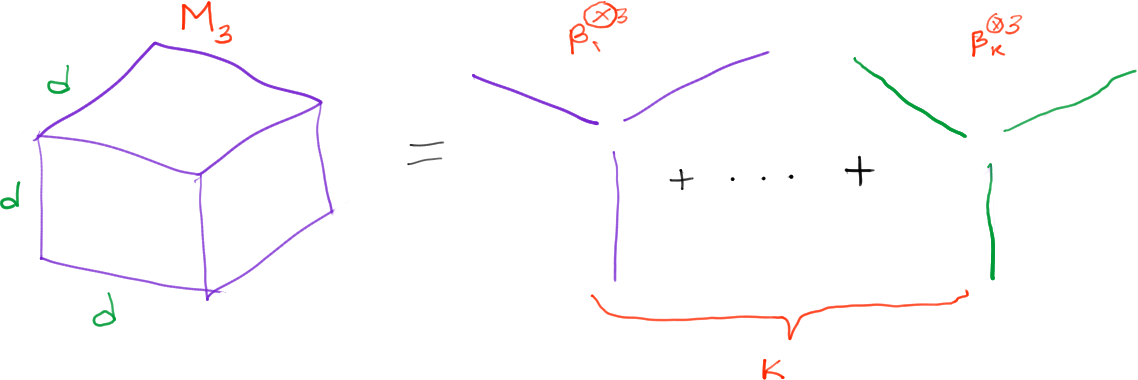
\includegraphics[width=\textwidth,height=6cm,keepaspectratio]{figures/tensor.png}
      };
  \end{tikzpicture}
\end{frame}

\begin{frame}
  \frametitle{Spectral Experts}

  \begin{canvas}
    % x, y
% Nodes
%\node[style=txt,anchor=south west] (data1) at (1cm,1cm) {$\left\{ x, y \right\}_{(x,y) \in \sD}$};
\node[style=txt] (data2) at (-4cm,1cm) {$\left\{ x\tp{2}, y^2 \right\}_{(x,y) \in \sD}$};
\node[style=txt,below=1cm of data2.center] (data3) {$\left\{ x\tp{3}, y^3 \right\}_{(x,y) \in \sD}$};

%\node[style=txt,anchor=south west] (m1) at (2cm,1cm) {$\E\left[\beta_h\right]$};
\node[style=txt] (m2) at (0cm,1cm) {$M_2$}; %{$\E\left[\beta_h\tp{2}\right]$};
\node[style=txt,below=1cm of m2.center] (m3) {$M_3$}; %{$\E\left[\beta_h\tp{3}\right]$};

\node[below=0.5cm of m2.center] (params-pos) {};
\node[style=txt,right=3.0cm of params-pos] (params) {$\pi, B$};

% Arrows
%\draw[-latex] (data1) -- (m1);
\draw[-latex] (data2) -- (m2);
\draw[-latex] (data3) -- (m3);

% Bias influence
%\draw[-latex,dashed,gray] (m1.east) -- ++(0.1cm,0) -- ++(0,-0.50cm) -- ++(-3.00cm,0) node (bias-1) {} -- ( bias-1 |- m3) -- (m3.west);

% Mean
\draw[-latex] (m2.east) -- ++(0.1cm,0) node (tf-1) {} -- (tf-1 |- params-pos) -- node[above,scale=0.5] {tensor factorization} (params);
\draw[-latex] (m3.east) -- ++(0.1cm,0) node (tf-2) {} -- (tf-2 |- params-pos) -- (params);

% Box for regression
\begin{pgfonlayer}{background}
%\draw[fill=blue,opacity=0.1,dashed] ($(data1.north east) + (-0.1cm,0.1cm)$) rectangle ($(m3.south west) + (0.1cm,-0.1cm)$);
\draw[fill=blue,opacity=0.1,dashed] ($(data2.north east) + (-0.1cm,0.1cm)$) rectangle ($(m3.south west) + (0.1cm,-0.1cm)$);
\end{pgfonlayer}

% tensor factorization
\begin{pgfonlayer}{background}
\draw[fill=green,opacity=0.1,dashed] ($(m2.north east) + (-0.1cm,0.1cm)$) rectangle ($(params.south west) + (0.1cm,-1.0cm)$);
\end{pgfonlayer}
\node (params-mid) at ($(params-pos) !.5! (params)$) {};
\point{reg-label}{($(data3) !.5! (m3) + (0, -1.0cm)$)};
\point{tf-label}{(params-mid |- reg-label)};



    \node[style=txt] at (reg-label) {{\color{blue}\bf low-rank} regression};
    \node[style=txt] at (tf-label) {tensor factorization};

    % Error bounds
    \node<2->[style=txt,below=0.1em of reg-label]{%
      $O\left( k\ 
      \hlmath{blue}{\|x\|^{12}}\
      \hlmath{DarkGreen}{\|\beta\|^{6}}\
      \hlmath{red}{\|\E[\epsilon^2]\|^{6}}
      \right)$};
    \node<3->[style=txt,below=0.1em of tf-label] {%
    $O\left( \frac{k \pi_{\max}^2}{\sigma_k(M_2)^5} \right)$};
  \end{canvas}
\end{frame}

\begin{frame}
  \frametitle{Experimental Insights}

  \begin{canvas}
    % x, y
    \node[anchor=west] (em) at (-0.5cm,-1.5cm) {%
      \includegraphics<1>[width=\textwidth,height=5cm,keepaspectratio]{figures/1-8-3.png}
      \includegraphics<2>[width=\textwidth,height=5cm,keepaspectratio]{figures/1-8-3-em.png}
      \includegraphics<3>[width=\textwidth,height=5cm,keepaspectratio]{figures/1-8-3-spec.png}
      \includegraphics<4->[width=\textwidth,height=5cm,keepaspectratio]{figures/1-8-3-specm.png}
      };
    % x, y
    \node[anchor=west, right=6cm of em] at (em.west) {%
      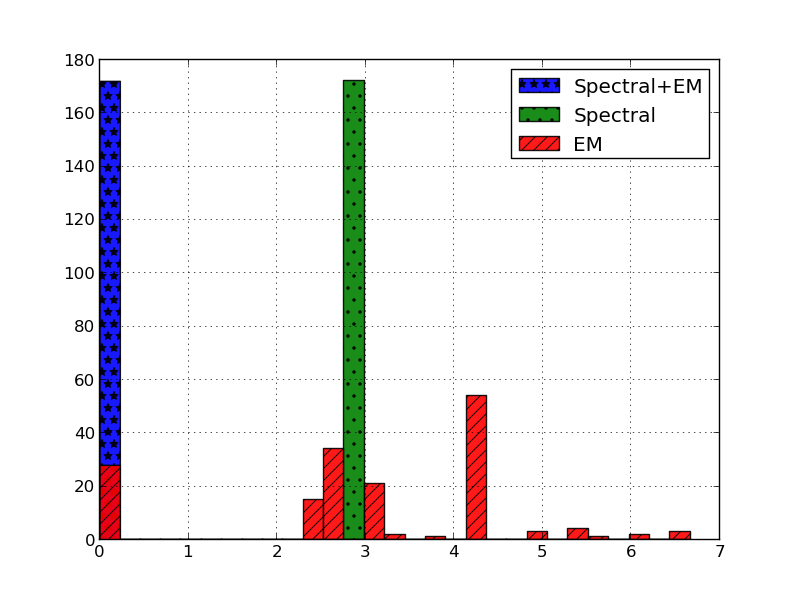
\includegraphics[width=\textwidth,height=5cm,keepaspectratio]{figures/hist.png}
    };

    \node[above=0.1 cm of em] {%
        $y = \beta^T 
            \begin{bmatrix} 
              1 \\
              t \\
              t^4 \\
              t^7
            \end{bmatrix} + \epsilon$
      };
  \end{canvas}
\end{frame}

\begin{frame}
  \frametitle{Experimental Insights}

\begin{small}
  \begin{tabular}{r r r c c c}
\hline
%$b$ & 
$d$ & $k$ & Spectral & EM & Spectral + EM \\
\hline
  %1 & 
  4 & 2 & 2.45 $\pm$ 3.68 & 0.28 $\pm$ 0.82 & {\bf 0.17 $\pm$ 0.57} \\
  %2 & 
  5 & 2 & 1.38 $\pm$ 0.84 & {\bf 0.00 $\pm$ 0.00} & {\bf 0.00 $\pm$ 0.00} \\
  %2 & 
  5 & 3 & 2.92 $\pm$ 1.71 & 0.43 $\pm$ 1.07 & {\bf 0.31 $\pm$ 1.02} \\
  %2 & 
  6 & 2 & 2.33 $\pm$ 0.67 & 0.63 $\pm$ 1.29 & {\bf 0.01 $\pm$ 0.01} \\
\hline
\end{tabular}
      \end{small}

\end{frame}

\begin{frame}
  \frametitle{Experimental Insights}

  \begin{tikzpicture}
    \node at (0,0) {%
      \includegraphics<1>[width=\textwidth,height=6cm,keepaspectratio]{figures/likelihood-mom.png}
      \includegraphics<2>[width=\textwidth,height=6cm,keepaspectratio]{figures/likelihood-mom-em1.png}
      \includegraphics<3>[width=\textwidth,height=6cm,keepaspectratio]{figures/likelihood-mom-em2.png}
    };
    \draw[-latex] (-6cm,-2.25cm) -- node[right,at end]{$-\log(p_{\theta}(x))$}  (-6cm,2cm);
    \draw[-latex] (-6cm,-2.25cm) -- node[above,at end]{$\theta$}  (5cm,-2.25cm);

    \node<2-> at (1.8cm,0.6cm) {$\hlmath{DarkGreen}{\theta_{spec}}$};
    \node<3-> at (0.3cm,-0.8cm) {$\hlmath{blue}{\theta^{*}}$};
  \end{tikzpicture}

\end{frame}


\begin{frame}
  \frametitle{Conclusions}
  \begin{itemize}
    \item {\bf Consistent estimator} for the mixture of linear regressions with {\bf polynomial sample and computational complexity}.
    \item<2-> Derive conditional moments using regression.
    \item<3-> Method of moment estimates can be a good initialization for EM.
  \end{itemize}
\end{frame}

\begin{frame}
  \frametitle{}
    Thank you.
\end{frame}

\end{document}

% TikZ
%\begin{canvas}
%  \node (img1) at (0,0) {\includegraphics[height=0.6\textheight,width=0.4\linewidth,keepaspectratio]{}};
%\end{canvas}

% Notes 
% \note[item]{}

% 2-column
% \begin{columns}
%   \begin{column}{0.48\textwidth}
%     \begin{itemize}
%         \item
%     \end{itemize}
%   \end{column}
%   \hfill
%   \begin{column}{0.48\textwidth}
%     \begin{itemize}
%         \item
%     \end{itemize}
%   \end{column}
% \end{columns}

% TikZ
%\begin{canvas}
%  \node (img1) at (0,0) {\includegraphics[height=0.6\textheight,width=0.4\linewidth,keepaspectratio]{}};
%\end{canvas}

% Notes 
% \note[item]{}

% 2-column
% \begin{columns}
%   \begin{column}{0.48\textwidth}
%     \begin{itemize}
%         \item
%     \end{itemize}
%   \end{column}
%   \hfill
%   \begin{column}{0.48\textwidth}
%     \begin{itemize}
%         \item
%     \end{itemize}
%   \end{column}
% \end{columns}

